\documentclass{article}
\usepackage[T2A]{fontenc}
\usepackage[english,russian]{babel}
\usepackage[utf8]{inputenc}
% \usetheme{Warsaw}
\usepackage{graphics}
\usepackage[demo]{graphicx}
\graphicspath{ {./images/} }
\usepackage{subfig}
\usepackage[utf8]{inputenc}
\usepackage{amsmath, amssymb}
\usepackage[export]{adjustbox}
\usepackage{caption}
\usepackage{subcaption}
\captionsetup{compatibility=false}

\title{Отчёт о проделанной работе}
\author{Лазар В. И.}

\begin{document}
\maketitle

\section{Проведённые исследования}

\subsection{Модель}

Программно реализована однопиковая модель \textbf{PBFTPK} с возможностью обучения на данных и генерации сэмплов с параметрами, подобранными при обучении. \newline

Сама модель устроена следующим образом:

$$
	C_{\tau}(t) = \begin{cases}
		\frac{F D k_a}{V_d (k_a - k_{el})} (e^{-k_{el} t} - e^{-k_a t}), t \le \tau \\
		C_{\tau}(\tau)e^{-k_el (t - \tau)}, t > \tau
	\end{cases}
$$
\begin{align*}
	 & C_{\tau}(t) - \text{концентрация декарства в крови}                            \\
	 & D > 0 - \text{объём дозы лекарства}                                            \\
	 & F > 0 - \text{биодоступная доля дозы}                                          \\
	 & V_d > 0 - \text{объём распределения лекарства}                                 \\
	 & k_a - \text{параметр всасывания вещества}                                      \\
	 & k_el - \text{параметр выведения вещества}                                      \\
	 & \tau > 0 - \text{время абсорбции}, C_{\tau}(\tau) = \sup_{t \ge 0} C_{\tau}(t)
\end{align*}

Реализована многопиковая модель:

$$
	C_n(t) = \sum_{i=1}^{n} C_{\tau_i}
$$


\subsection{Метрика}

В качестве метрики для оценки моделей большинство уже реализованных алгоритмов используют метрику \[
	\frac{1}{n}\sum_{i=1}^{n} (f(t_i) - X(t_i))^2
\] Было решено использовать несколько иную метрику: \[
	L(f, \alpha) = \frac{1}{n}\sum_{i=1}^{i_0-1} |f(t_i) - X(t_i)| +
	\frac{1}{n}\sum_{i=i_0}^{n} \alpha|f(t_i) - X(t_i)|
\], где \[
	t_{i_0} \approx \tau
\] в силу того, что она чувствительнее к ошибке модели после достижения времени абсорбции. Соответственно, для случая многопиковой модели метрика выглядит следующим образом: \[
	L_{mul}(f)  = \sum_{i=0}^{n} L(f, \alpha_i)
\]

Также для улучшения качества модели было принято решение использовать MinMaxScaler

\subsection{Исследование моментных характеристик остатков}

Здесь и далее будем действовать в предположении о том, что величина
\[
	X(t) - f(t)
\], где X(t) - исходный случайный процесс, а f(t) - тректория предсказанная моделью, является процессом Леви

Для получения более точного вида процесса было решено исследовать матожидание и стандартное отклонение проекций процесса остатков \newline\newline

Для тестирования использовалась однопиковая модель с $\alpha=7$ \newline

Получен следующий график поведения для матожидания

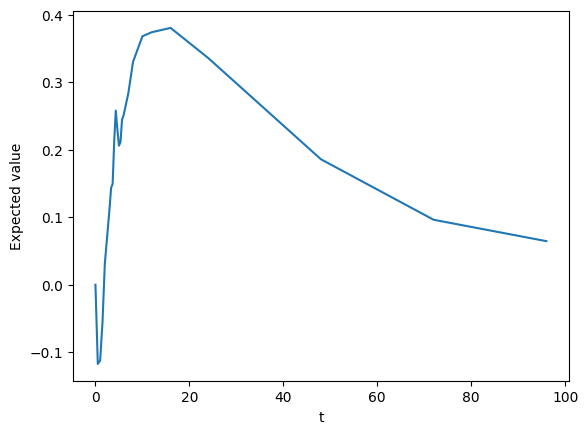
\includegraphics[width=0.7\textwidth, left]{mean.png}

И для дисперсии

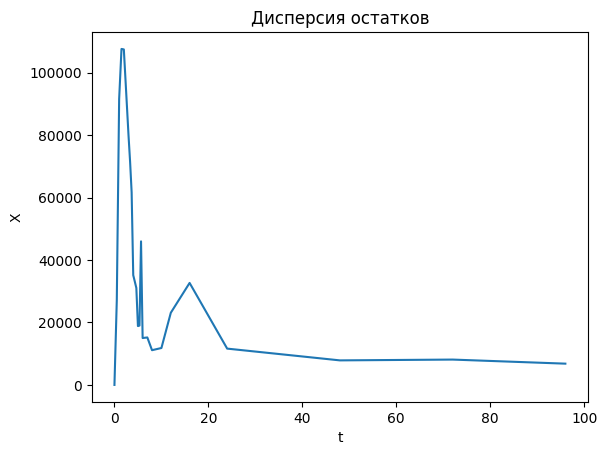
\includegraphics[width=0.7\textwidth, left]{var.png}

Видно, что модель довольно сильно ошибается до момента абсорбции, что логично следует из выбранных гиперпараметров модели

\subsection{Исследование поведения исходного процесса}

Здесь показаны одни из типовых случаев процессов, на которых модель значительно ошибается ошибается

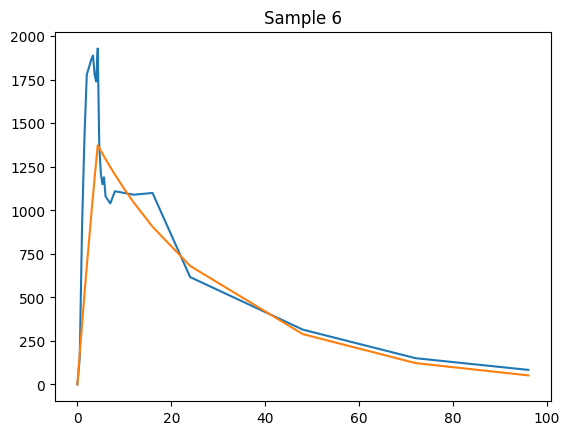
\includegraphics[width=0.6\textwidth]{example4_1.png} \newline
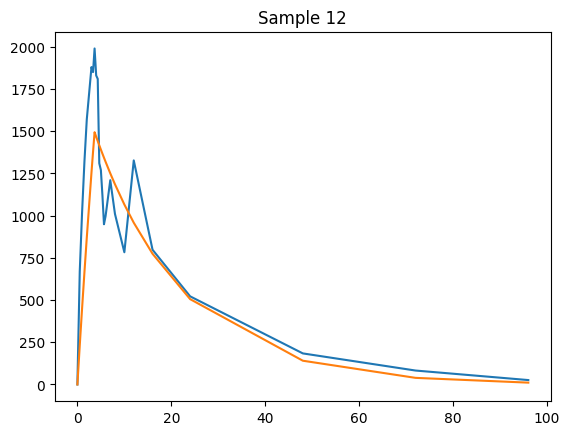
\includegraphics[width=0.6\textwidth]{example5_1.png} \newline
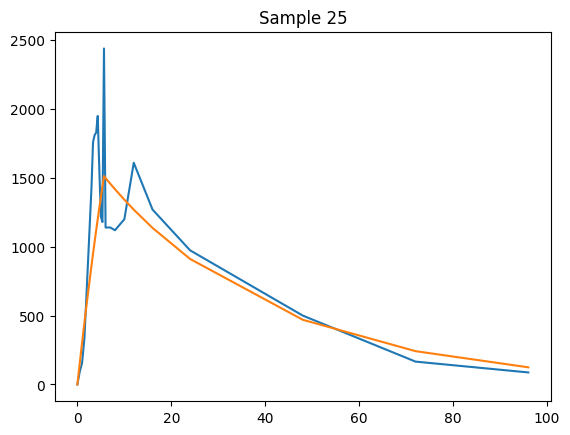
\includegraphics[width=0.6\textwidth]{example6_1.png} \newline

В среднем даваемая моделью оценка выглядит так:

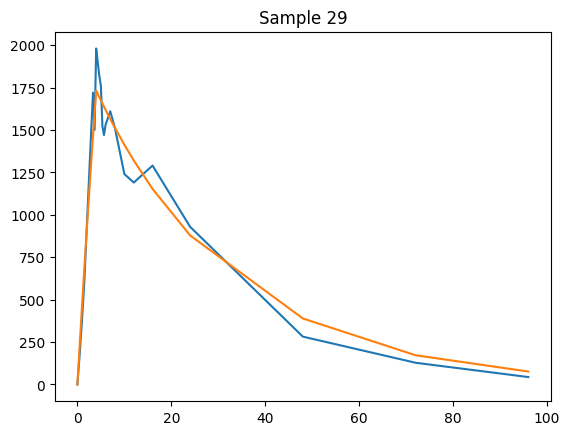
\includegraphics[width=0.6\textwidth]{example1_1.png} \newline
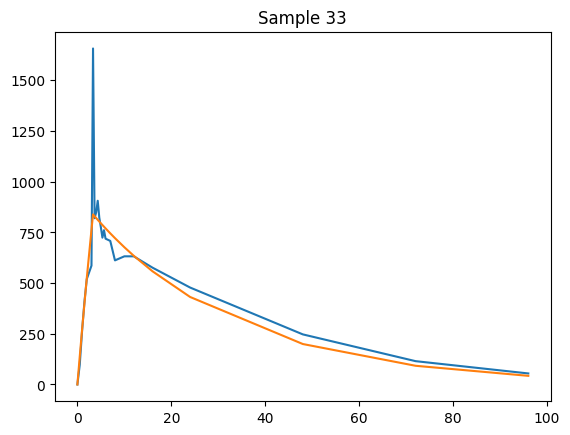
\includegraphics[width=0.6\textwidth]{example2_1.png} \newline
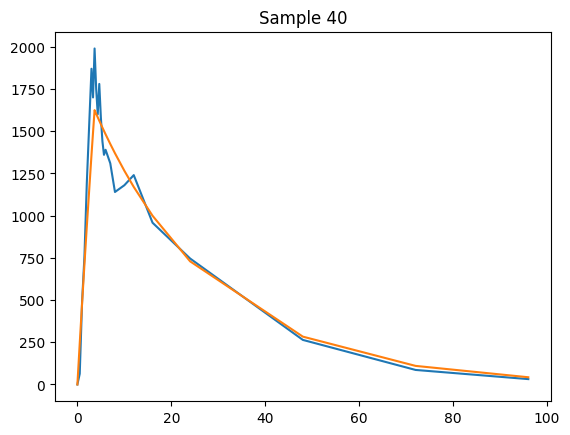
\includegraphics[width=0.6\textwidth]{example3_1.png} \newline

\section{Гипотезы и планы}

\subsection{Доработка модели}

Сейчас многопиковая модель показывает себя в среднем хуже однопиковой с параметром регуляризации и нуждается в существенной программной доработке. Возможно, имеет смысл поиск других способов обнаружения пиков процесса

\section{Исследование поведения процесса остатков}

Было получено, что при $\lim_{t \to +\infty} \mathbb{E} r(t) \approx 0$, а также $\mathbb{D} r(t) \approx const$ при $t > \tau$. Это существенно сужает круг возможных семейств процессов. Учитывая, что в данной модели процесс остатков представляется процессом Леви, можно исключить некоторые слагаемые из декомпозиции Леви-Ито: \newline $ X_t = \sigma B_t + at + Y_t + Z_t $

\end{document}
